\begin{center}
	\LARGE
	Uden hjælpemidler
\end{center}
\begin{opgavetekst}{Opgave 1}
\end{opgavetekst}
\begin{delopgave}{1}
	Reducer udtrykket $(a + b)(a - b) + b^2 - 2a^2$.
\end{delopgave}
%
%
%
%
%
%
\begin{opgavetekst}{Opgave 2}
\end{opgavetekst}
\begin{delopgave}{1}
	Bestem grænseværdien for følgende $0/0$-udtryk:
	\begin{align*}
		\lim_{x \to 4} \frac{x^2 - 16}{x - 4}.
	\end{align*}
\end{delopgave}
%
%
%
%
%
\begin{opgavetekst}{Opgave 3}
	En funktion $f$ er givet ved 
	\begin{align*}
		f(x) = \ln(x^2).
	\end{align*}
\end{opgavetekst}
\begin{delopgave}{1}
	Bestem $f'(x)$.
\end{delopgave}
\begin{delopgave}{2}
	Bestem ligningen for tangenten til $f$ i punktet $P(1,f(1))$.
\end{delopgave}
%
%
%
%
%
\begin{opgavetekst}{Opgave 4}
	På Figur \ref{fig:arealer} kan vi se grafen for en funktion $f$ samt arealet $A$, der afgrænses af grafen for $f$ og $x$-aksen. Funktionen $f$ har forskriften
	\begin{align*}
		f(x) = x^3 - x^2 - 2x.
	\end{align*}
	\begin{figure}[H]
		\centering
		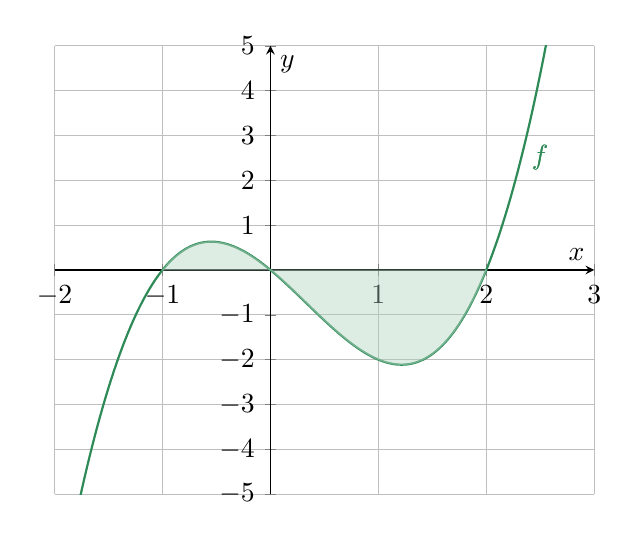
\begin{tikzpicture}
		\begin{axis}[
		axis lines = middle,
		xmin = -2, xmax = 3,
		ymin = -5, ymax = 5,
		xlabel = {$x$}, ylabel = {$y$},
		xtick = {-2,-1,0,...,3},
		ytick = {-5,-4,...,5},
		grid = both
		]
			\addplot[color = SeaGreen, thick, domain = -2:3, samples = 200] {x^3 - x^2 - 2*x};
			\filldraw[domain = -1:2, color = SeaGreen!40, opacity = 0.4, samples = 200] (axis cs: -1,0) -- plot (axis cs: \x, \x*\x*\x - \x*\x - 2*\x) -- (axis cs: 2,0) -- cycle;
			\node[color = SeaGreen] at (axis cs: 2.5,2.5) {$f$};
			\node[color = SeaGreen] at (axis cs: 2.5,2.5) {$f$};
		\end{axis}
		\end{tikzpicture}
		\caption{Graf for funktionen $f$ med arealet $A$ markeret.}
		\label{fig:arealer}
	\end{figure}
	\phantom{h}
\end{opgavetekst}
\begin{delopgave}{1}
	Vis, at arealet $A = \frac{37}{12}$.
\end{delopgave}
%
%
%
%
%
\begin{opgavetekst}{Opgave 5}
	En trekant $\triangle ABC$ er givet på Figur \ref{fig:trekant}.
	\begin{figure}[H]
		\centering
		\begin{tikzpicture}
			\draw[color = SeaGreen, thick] (0,0) -- (10*0.6,0) node[midway, anchor = north] {$10$} 
			node[pos = 0, anchor = north east] {$A$} node[pos = 1, anchor = north west] {$C$};
			\draw[color = SeaGreen, thick] (0,0) -- (5*0.6,6.25*0.6) node[midway, anchor = south east] {$8$}
			node[pos = 1, anchor = south] {$B$};
			\draw[color = SeaGreen, thick] (5*0.6,6.25*0.6) -- (10*0.6,0) node[midway, anchor = south west] {$8$};
		\end{tikzpicture}
		\caption{Trekanten $\triangle ABC$.}
		\label{fig:trekant}
	\end{figure}
	\phantom{h}
\end{opgavetekst}
\begin{delopgave}{1}
	Vis, at $\cos(\angle A) = \frac{5}{8}$.
\end{delopgave}
%
%
%
%
%
\newpage
\begin{opgavetekst}{Opgave 6}
	To vektorer $\vv{a}$ og $\vv{b}$ er givet ved
	\begin{align*}
		\vv{a} = \begin{pmatrix}
			t \\ -1
		\end{pmatrix}
	\quad \textnormal{og} \quad
		\vv{b} = \begin{pmatrix}
			t-1 \\ 6
		\end{pmatrix}.
	\end{align*}
\end{opgavetekst}
\begin{delopgave}{1}
	Bestem de værdier for $t$, så $\vv{a}$ og $\vv{b}$ er ortogonale.
\end{delopgave}
%
%
%
%%
%
\begin{opgavetekst}{Opgave 7}
	En cirkel $c$ er givet ved ligningen
	\begin{align*}
		c:\  x^2 + y^2 - 4x - 6y + 9 = 0.
	\end{align*}
\end{opgavetekst}
\begin{delopgave}{1}
	Bestem centrum og radius for cirklen $c$.
\end{delopgave}	
%
%
%%%%%%%%%%%%%%%
%
%
\newpage
\begin{center}
	\LARGE
	Med hjælpemidler
\end{center}
%
%
%
\begin{opgavetekst}{Opgave 8}
	To linjer $l$ og $m$ er givet ved henholdsvis
	\begin{align*}
		&l: \ 5x + 19y = 12, \\
		&m: \ 10x -10y = 29.
	\end{align*}
\end{opgavetekst}
\begin{delopgave}{1}
	Bestem skæringspunktet mellem $l$ og $m$.
\end{delopgave}
\begin{delopgave}{2}
	Brug en formel til at bestemme den spidse vinkel mellem $l$ og $m$.
\end{delopgave}
%